\begin{frame}[c]
  \frametitle{Case VI : Waste Package Failure Time and Diffusion Coefficient}

To investigate the effect of the waste package failure time, it was varied over 
five magnitudes from one thousand to ten million years. Simultaneously, the reference 
diffusivity was varied over the eight magnitudes between $1\times10^{-8}$ and 
$1\times10^{-15}$ in order to determine the correlation between increased 
radionuclide mobility and the waste package lifetime. 
\begin{table}[ht!]
\centering
\footnotesize{
\begin{tabular}{|l|l|l|r|r|}
\multicolumn{5}{c}{\textbf{Simulation Cases}}\\
\hline
\textbf{Case} & \textbf{Parameter} & \textbf{Units} & \textbf{Min. Value} & \textbf{Max. Value}\\
\hline 
VI    & $t_{WPFail}$        & $[yr]$         & $10^3$    &  $10^7$ \\
      & $D_{eff}$           & $[m^2\cdot s^{-1}]$       & $10^{-8}$    &  $10^{-5}$ \\
\hline
\end{tabular}
\caption{Each dual and single parameter simulation case had 40 simulation 
groups of 100 realizations each.}
\label{tab:Cases}
}
\end{table}


\end{frame}

\begin{frame}[c]
  \frametitle{Case VI : Waste Package Failure Time and Diffusion Coefficient}

For the clay repository, the waste package failure time is entirely irrelevant 
until waste package failure times reach the million or ten million year time 
scale. 

\begin{figure}[ht!]
\centering
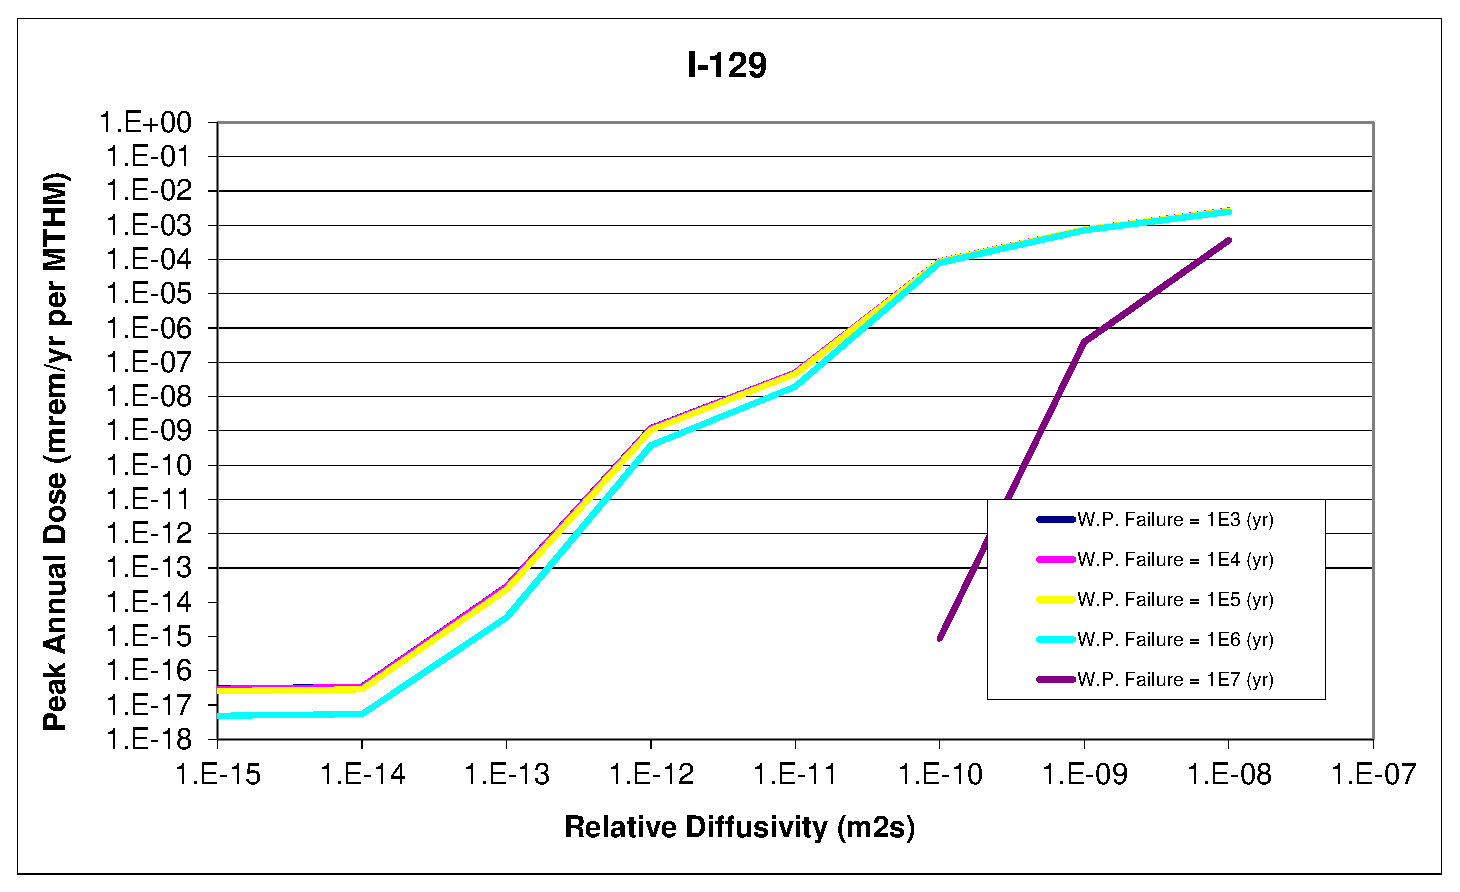
\includegraphics[width=0.8\textwidth]{WPFailExtended/I-129.eps}
\caption{$^{129}I$ waste package failure time sensitivity. }
\label{fig:WPFailI129}
\end{figure}
\end{frame}

\begin{frame}[c]
  \frametitle{Case VI : Waste Package Failure Time and Diffusion Coefficient}

\begin{figure}[ht!]
\centering
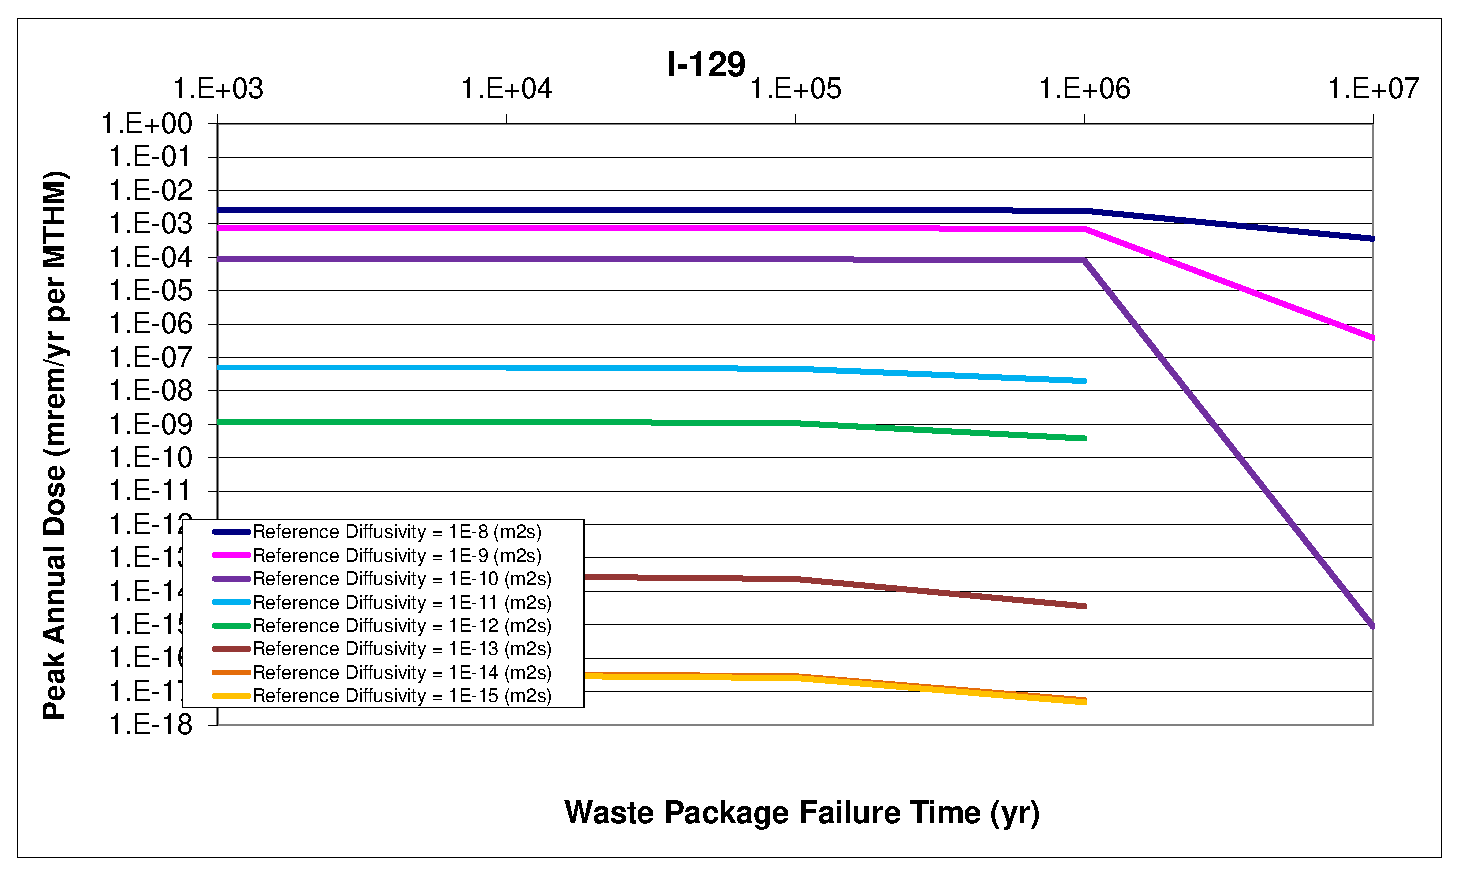
\includegraphics[width=0.8\textwidth]{WPFailExtended/I-129-WPFail.eps}
\caption{$^{129}I$ waste package failure time sensitivity. }
\label{fig:WPFailI129}
\end{figure}
\end{frame}


